\documentclass[../main.tex]{subfiles}

\begin{document}
\begin{problema}
	Considera un fluido ideal, donde \(\bm{\sigma} = -p \bm{I}\),
	y fuerza de cuerpo conservativa \(\bm{\mathrm{f}} = - \nabla{\phi}\).

	\begin{enumerate}
		\item Para flujo estacionario, demuestra que:
		      \begin{equation*}
			      \nabla \cdot{\Biggl(\bm{\mathrm{v}}\Biggl(\dfrac{v^{2}}{2} + \phi\Biggr)\Biggr)}
			      + \dfrac{1}{\rho}\bm{\mathrm{v}} \cdot \nabla{p} = 0.
		      \end{equation*}
		\item Para flujo estacionario e irrotacional (i.e. \(\nabla \mul\bm{\mathrm{v}} = 0\)),
		      demuestra que:

		      \begin{equation*}
			      \nabla{\Biggl(\dfrac{v^{2}}{2} + \phi\Biggr)} + \dfrac{1}{\rho}\nabla{p} = 0.
		      \end{equation*}
		\item Determina la velocidad y el gasto volumétrico del fluido en la salida
		      de la boquilla en la pared del depósito mostrado en la figura
		      (\(d \ll D\), con \(D\) el diámetro del contenedor.)
	\end{enumerate}

	\begin{figure}[htb]
		\centering
		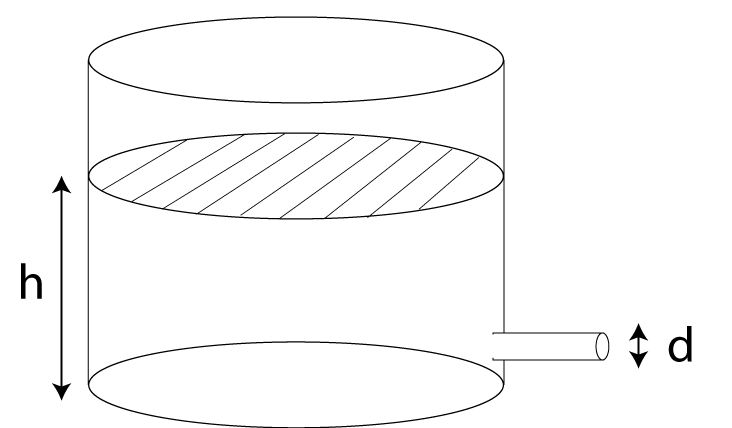
\includegraphics[width=0.45\textwidth]{figs/problema02.png}
	\end{figure}
\end{problema}
\end{document}
